% !TEX root = ../diz.tex
The definition of a P system is based on the notion of \index{Membrane!structure} membrane structure \cite{Besozzi:PhD:2004}, which is introduced in terms of the language $MS$ over the alphabet $\{[, ]\}$, consisting of the strings recurrently defined as follows:
\begin{enumerate}
  \item $[]\in MS$,
  \item if $\mu_1, \ldots, \mu_n \in MS$, then $[\mu_1\ldots\mu_n] \in MS$,
  \item nothing else is in $MS$.
\end{enumerate}

We assume that each pair of well matching parentheses $[]$ can be labelled in a one-to-one manner by an integer in the set $1\ldots m$, e.g. $[[]_2[]_3]_1$.

We define now an equivalence relation over the elements of $MS$: we write $x\sim y$ if and only if:
\begin{enumerate}
  \item $x=[]_i$ and $y=[]_i$,
  \item $x=[\mu_1\ldots\mu_n]_j$, $y=[\xi_1\ldots\xi_n]_j$ and $\mu_i\sim\xi_{p(i)}$ for every $i$ and for some permutation $p$.
\end{enumerate}

Thus, the order of parentheses is irrelevant as long as they are at the same hierarchical level. The set of equivalence classes with respect to the equivalence relation $\sim$ is denoted by $\overline{MS}$.

\begin{definition}
  Any element in $\overline{MS}$ is called a {\bf membrane structure}.
\end{definition}

\begin{definition}
  Each pair of matching parentheses $[]$ appearing in a membrane structure $\mu$ is called a \index{Membrane} {\bf membrane}.
\end{definition}

\begin{definition}
  The external membrane of a membrane structure is called the \index{Membrane!skin} {\bf skin membrane}.
\end{definition}

\begin{definition}
  Any membrane without any other membrane inside (appearing in a membrane structure in the form $[]$) is called an \index{Membrane!elementary} {\bf elementary membrane}.
\end{definition}

\begin{definition}
  The number of membranes in $\mu$ is called the {\bf degree} of $\mu$ and it is denoted by $deg(\mu)$.
\end{definition}

\begin{definition}
  The depth of a membrane structure $\mu$, $dep(\mu)$, is recurrently defined as:
  \begin{enumerate}
    \item if $\mu = []$, then $dep(\mu) = 1$;
    \item if $\mu = [\mu_1\ldots\mu_n]$ for some $\mu_1, \ldots, \mu_n\in MS$, then $dep(\mu) = 1 + max\{dep(\mu_i\} | 1\leq i\leq n)$.
  \end{enumerate}
\end{definition}

Each membrane determines a compartment, also called region, the space delimited from above by it and from below by the membranes placed directly inside, if any exists. The correspondence membrane-region is one-to-one, that is why we sometimes use interchangeably these terms.


Next step is inserting objects into regions and adding them the possibility to evolve and communicate according to certain specified rules.

\begin{definition}
\label{def:evolution_rule}
  An {\bf evolution rule} over an alphabet $\Sigma$ is a pair $(u,v)$, which will be written as $u\rightarrow v$, where $u$ is a string over $\Sigma$ and $v=v^\prime$ or $v=v^\prime\delta$, where $v^\prime$ is a string over $\Sigma\times(\{here, out\}\cup\{in_j|1\leq j\leq m\})$ and $\delta$ is a special symbol not in $\Sigma$.
\end{definition}

An example of such rule is $ab^2\rightarrow (a,here)(b,in_3)(c,out)(c,here)$. An evolution rule specifies for each object on the right side, whether it stays in the current region, moves through a membrane to the parent region or through a membrane to one of the child regions.

\begin{definition}
  For an evolution rule $r: u\rightarrow v$, the size of multiset $u$ is called the {\bf radius} of $r$.
\end{definition}

Note that the strings $u, v$ are understood as representations of multisets over $\Sigma$, in a sense from section \ref{sec:multisets}.

We are now ready to proceed with a formal definition of a P system of degree $m$.

\begin{definition}
  A \index{P systems!definition} {\bf P system} is a tuple $$\Pi = (\Sigma, \mu, w_1, w_2,\ldots , w_m, R_1, R_2,\ldots , R_m),$$ where:
  \begin{itemize}
    \item $\Sigma$ is the alphabet of objects,
    \item $\mu$ is a membrane structure consisting of $m$ membranes labeled with numbers $1,2,\dots,m$,
    \item $w_1,w_2,\ldots w_m$ are multisets of objects from $\Sigma$ initially present in the regions $1,2,\ldots,m$ of the membrane structure,
    \item $R_1,R_2,\ldots R_m$ are finite sets of evolution rules associated with the regions $1,2,\dots,m$ of the membrane structure.
  \end{itemize}
\end{definition}

Some more remarks about the definition of a P system are to be given, before explaining its functioning as a computing device.

Any of the initial multisets $w_1, w_2,\dots , w_m$ can be empty as well as any of the sets of evolution rules $R_1,R_2,\ldots R_m$.

The $(m+1)$-tuple $(\mu, w_1,w_2,\ldots w_m)$ constitutes the initial configuration of the P system $\Pi$. In general, the configuration is represented by the membrane structure of $\Pi$and the multisets of objects in the regions.

\begin{definition}
  A \index{P systems!configuration} {\bf configuration} of a P system $\Pi$ is an $(m+1)$-tuple $(\mu^\prime, w^\prime_1,w^\prime_2,\ldots w^\prime_m)$, where $\mu^\prime$ is a membrane structure and $w^\prime_1,w^\prime_2,\ldots w^\prime_m$ are multisets over $\Sigma$ present in the regions $1,2,\ldots,m$ of $\mu^\prime$.
\end{definition}

Note that the membrane structure can be different from the initial membrane structure, according to the dissolving action, which will be explained later.

\begin{definition}
  A rule $(r: u\rightarrow v)\in R_i$ is {\bf applicable} in the configuration $C = (\mu^\prime, w^\prime_1,w^\prime_2,\ldots w^\prime_m)$ of the P system $\Pi$, iff the following conditions are fulfilled:
  \begin{enumerate}
    \item $u\subseteq w^\prime_i$,
    \item for any object, which appears in $v$ in the form $(a, in_j)$ there is a membrane $j$ directly inside $i$,
    \item if $v=v^\prime\delta$, then $i$ is not the skin membrane.
  \end{enumerate}
\end{definition}

\begin{definition}
  The {\bf result of the application of the rule} $r: u\rightarrow v\in R_i$ in the configuration $C = (\mu^\prime, w^\prime_1,w^\prime_2,\ldots w^\prime_m)$ of the P system $\Pi$ is determined by the following prescription:
  \begin{itemize}
    \item the multiset $u$ is subtracted from $w_i$;
    \item if an object appears in $v$ in the form $(a, here)$, then it remains in the same region $i$ (the indication here will often be omitted);
    \item if an object appears in $v$ in the form $(a, out)$, then it exits the membrane $i$ and becomes an element of the region immediately outside it. If the membrane $i$ is the skin membrane, then the object leaves the system and it will never come back;
    \item if an object appears in $v$ in the form $(a,in_j)$ and $j$ a membrane immediately inside $i$, then the object $a$ is added to the multiset $w^\prime_j$. If it is not a membrane immediately inside $i$, then the application of the rule is not allowed;
    \item if the symbol $\delta$ appears in $v$, then the membrane $i$ is removed (we say it is dissolved) from $\mu^\prime$ and, at the same time, the multiset $w^\prime_i$ is added to the region immediately outside of the membrane $i$. The dissolving of the skin membrane is not allowed.
  \end{itemize}
\end{definition}

For better understanding of this process, we present an algorithm for the rule application \vpageref[below]{alg:application_of_a_rule_in_a_p_system}.

\begin{algorithm}
  \caption{Application of a single rule in a P system}\label{alg:application_of_a_rule_in_a_p_system}
  \begin{algorithmic}[1]
    \Procedure{RuleAplication}{applicable rule $u\rightarrow v\in R_i$, configuration $C = (\mu^\prime, w^\prime_1,w^\prime_2,\ldots w^\prime_m)$}
      \State $w_i := w_i - u$
      \ForAll{$(a, here)\in v$}
        \State $w_i := w_i + a$
      \EndFor
      \ForAll{$(a, out)\in v$}
        \State $w_{parent(i)} := w_{parent(i)} + a$
      \EndFor
      \ForAll{$(a, in_j)\in v$}
        \State $w_j := w_j + a$
      \EndFor
      \If{$v = v^\prime\delta$}
        \State $w_{parent(i)} := w_{parent(i)} + w_i$
        \State $w_i := \text{empty multiset}$
      \EndIf
    \EndProcedure
  \end{algorithmic}
\end{algorithm}

All these operations are performed in a maximal parallel mode: inside each region all applicable rules $u\rightarrow v$ are used over all occurrences of multisets $u$, and all regions are processed at the same time. Hence, the parallelism is maximal at both a global and a local level: the global level involves all membranes at the same time, the local level involves all evolution rules and all objects inside each region.

\begin{definition}
  A multiset of rules $$\rho: \bigcup_{1\leq i\leq m} R_i \rightarrow \mathbb N$$ is {\bf simultaneously applicable} in the configuration $C = (\mu^\prime, w^\prime_1,w^\prime_2,\ldots w^\prime_m)$ of the P system $\Pi$, iff the following conditions are fulfilled:
  \begin{enumerate}
    \item for any membrane with label $1\leq i\leq m$, there is enough objects to allow simultaneous application of rules: $$ \bigcup_{(r: u\rightarrow v)\in supp(\rho)\cap R_i} \rho(r)\cdot u \subseteq w^\prime_i$$,
    \item for any membrane with label $1\leq i\leq m$, any rule $u\rightarrow v\in supp(\rho)\cap R_i$, any object, which appears in $v$ in the form $(a, in_j)$ there is a membrane $j$ directly inside $i$,
    \item for the skin membrane $i$, any rule $r: u\rightarrow v^\prime\delta\in R_i$ has no occurence in the multiset: $\rho(r)=0$.
  \end{enumerate}  
\end{definition}

The multiset of simultaneously applicable rules is maximal iff adding more rules to the multiset make it not simultaneously applicable. Simultaneous application of a multiset of rules arises no contradictions:

\begin{itemize}
  \item if there is both $(a, out)$ and $\delta$ present in $v$, the object $a$ ends up in the parent region,
  \item if there is a rule from $R_i$ with $v$ containing $(a,in_j)$ and a rule from $R_j$ with $v$ containing $\delta$, the object $a$ ends up in the region $i$ 
\end{itemize}

\begin{definition}
  A {\bf computation step} of a P system is a relation $\Rightarrow$ on the set of configurations such that $C_1 \Rightarrow C_2$ iff there is a nonempty maximal multiset of simultaneously applicable rules, which, applied to $C_1$, can result in $C_2$.
\end{definition}

Because there can be more than one maximal multiset, for a configuration $C_1$ there can be multiple possible results $C_2$, so one of them is nondeterministically chosen.

Starting from the initial configuration and applying the rules in the way described above, we obtain a sequence of transition among configurations; such a sequence is called a computation of $\Pi$.

\begin{definition}
  An {\bf infinite computation} of a P system is an infinite sequence of configurations $\{C_i\}_0^\infty$ such that $C_0$ is the initial configuration and $C_i\Rightarrow C_{i+1}$ for all $0\leq i$.
\end{definition}

\begin{definition}
  A {\bf finite computation} of a P system is a sequence of configurations $\{C_i\}_0^n$ such that $C_0$ is the initial configuration and $C_i\Rightarrow C_{i+1}$ for all $0\leq i<n$.
\end{definition}

\begin{definition}
  A {\bf halting configuration} $C$ of a P system is a configuration with no applicable rule.
\end{definition}

When no rule is applicable, there is only one maximal multiset of simultaneously applicable rules: an empty multiset, so there is no configuration $C^\prime$ such that $C\Rightarrow C^\prime$.

\begin{definition}
  A {\bf halting computation} of a P system is a finite computation ending with a halting configuration.
\end{definition}

% Result of a computation

There are multiple possible ways of assigning a result of a computation \cite{Besozzi:PhD:2004}. We present two of them:

\begin{enumerate}
    \item By considering the multiplicity of objects present in a designated membrane in a halting configuration. In this case we obtain a vector of natural numbers. We can also represent this vector as a multiset of objects or as Parikh image of a string.
    \item By concatenating the symbols which leave the system, in the order they are sent out of the skin membrane. If several symbols are expelled at the same time, then any ordering of them is assumed. In this case we generate a string.
\end{enumerate}

The result of a computation is clearly only one multiset or a string, but for one initial configuration there can be multiple possible computations. It follows from the fact that there exist more than one maximal multiset of rules that can be applied in each step. Aggregating the results of possible computations a P system defines a language or a Parikh image of a language. 

\begin{example}
  The P system in figure \ref{fig:p_system_fibonacci} computes a Fibonacci sequence. Maximal parallelism enforces the simultaneous movement of objects between regions 1 and 2. Every second step the number of occurences of the object $e$ in the skin membrane constitutes the following item in Fibonacci sequence. The P system has only one computation, which is infinite.
\end{example}

\begin{figure}[ht]
  \centering
  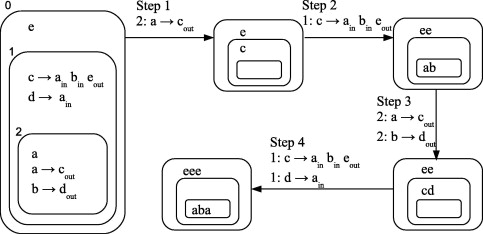
\includegraphics[width=0.8\textwidth]{img/p_system_fibonacci.jpg}
  \caption{P system computing a Fibonacci sequence \cite{Buiu201233PSystemFibonacci}}
  \label{fig:p_system_fibonacci}
\end{figure}

% TODO: quality vs quantity aspects.